\documentclass[12pt,a4paper]{article}
\usepackage[utf8]{inputenc}
\usepackage[T1]{fontenc}
\usepackage{amsmath, amssymb, graphicx, listings, caption}
\usepackage{xcolor}
\usepackage{hyperref}
\hypersetup{
    colorlinks=true,
    linkcolor=blue,
    filecolor=magenta,      
    urlcolor=cyan,
    pdftitle={MNIST Neuronales Netzwerk Bericht},
    pdfpagemode=FullScreen,
}
\lstset{
    basicstyle=\ttfamily\small,
    backgroundcolor=\color{lightgray!20},
    frame=single,
    keywordstyle=\color{blue},
    commentstyle=\color{green!70!black},
    stringstyle=\color{orange},
    showstringspaces=false,
    breaklines=true,
    tabsize=2,
    numbers=left,
    numberstyle=\tiny,
    numbersep=5pt,
    language=Python
}

\title{\textbf{Bericht zur Implementierung eines neuronalen Netzwerks zur MNIST-Klassifikation}}
\author{Luna Schätzle}
\date{\today}

\begin{document}

\maketitle

\section*{Aufgabenbeschreibung}
In Aufgabe 5 haben wir ein neuronales Netzwerk implementiert, um die MNIST-Datenbank zu klassifizieren. Die MNIST-Datenbank besteht aus 60.000 Trainings- und 10.000 Testbildern. Jedes Bild umfasst $28 \times 28$ Pixel und stellt eine handgeschriebene Ziffer von 0 bis 9 dar. Das Ziel war es, ein neuronales Netzwerk zu erstellen, das diese Ziffern zuverlässig klassifizieren kann.

Die Aufgabe erforderte die Implementierung eines vollständigen Workflows, einschließlich der Datenvorverarbeitung, dem Design der Netzwerkarchitektur, dem Trainieren des Modells, der Leistungsevaluierung und der Verwendung des trainierten Modells für Vorhersagen.

\section*{Datenladen}
Der erste Schritt bestand darin, den MNIST-Datensatz für das Modell zu laden. Die Funktion \texttt{load\_data()} wurde implementiert, um den Datensatz zu laden und die Trainings- sowie Testdaten zurückzugeben.

\subsection*{Code-Implementierung}
\begin{lstlisting}
import numpy as np
import tensorflow as tf
from tensorflow.keras.datasets import mnist

# MNIST-Datensatz laden
(x_train, y_train), (x_test, y_test) = mnist.load_data()

# Datensatzdimensionen ausgeben
print(f"x_train shape: {x_train.shape}")
print(f"y_train shape: {y_train.shape}")
print(f"x_test shape: {x_test.shape}")
print(f"y_test shape: {y_test.shape}")
\end{lstlisting}

\subsection*{Datensatzanalyse}
Der MNIST-Datensatz besteht aus Graustufenbildern, bei denen die Pixelwerte zwischen 0 und 255 liegen. Um die Verarbeitung für das neuronale Netzwerk zu vereinfachen, wurden die Pixelwerte auf den Bereich [0, 1] normalisiert, indem sie durch 255 geteilt wurden. Diese Normalisierung stellt sicher, dass das Netzwerk effizient arbeiten kann, ohne auf Probleme durch große Eingabewerte zu stoßen.

\subsection*{Visualisierung}
Ein Beispielbild aus dem Trainingsdatensatz wird unten dargestellt, zusammen mit Beispielbildern aus jeder Ziffernkategorie:

\begin{figure}[h!]
    \centering
    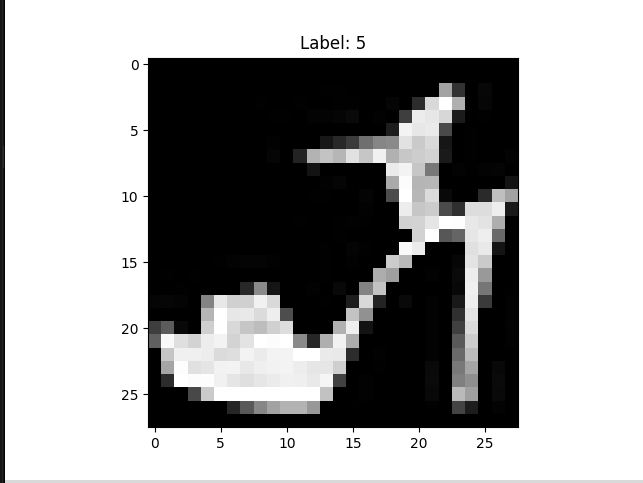
\includegraphics[width=0.6\textwidth]{image-1.png}
    \caption{Beispielbild aus dem Trainingsdatensatz}
    \label{fig:example-image}
\end{figure}

\begin{figure}[h!]
    \centering
    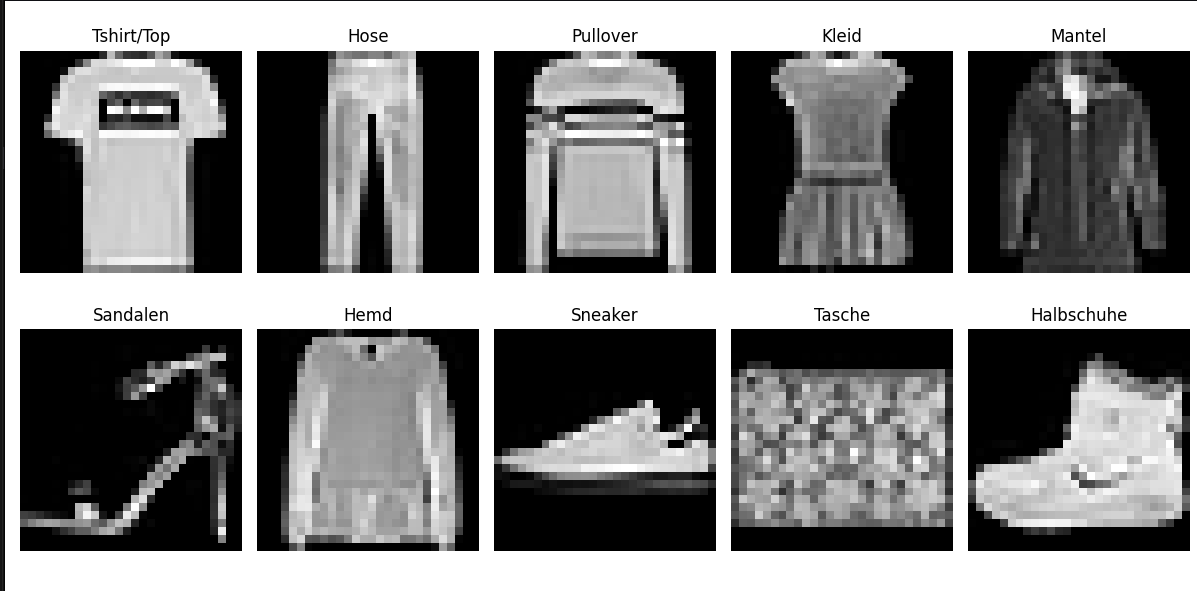
\includegraphics[width=0.8\textwidth]{image-2.png}
    \caption{Beispielbilder aus allen Ziffernkategorien}
    \label{fig:sample-images}
\end{figure}

\newpage

\section*{Modellarchitektur}
Das neuronale Netzwerk wurde mithilfe von Keras implementiert. Die Architektur umfasst:
\begin{itemize}
    \item Eine Eingabeschicht für $28 \times 28$ aufbereitete Pixel.
    \item Sechs dichte (vollständig verbundene) Schichten mit ReLU-Aktivierungsfunktion.
    \item Eine finale Ausgabeschicht mit Softmax-Aktivierung für 10 Klassen.
\end{itemize}



\subsection*{Code-Implementierung}
\begin{lstlisting}
from tensorflow.keras import models, layers

model = models.Sequential([
    layers.Input(shape=(28 * 28,)),
    layers.Dense(512, activation='relu'),
    layers.Dense(256, activation='relu'),
    layers.Dense(128, activation='relu'),
    layers.Dense(24, activation='relu'),
    layers.Dense(10, activation='relu'),
    layers.Dense(10, activation='softmax')
])
\end{lstlisting}

\subsection*{Modelzusammenfassung}
\begin{verbatim}
Model: "sequential"
┏━━━━━━━━━━━━━━━━━━━━━━━━━━━━━━━━━┳━━━━━━━━━━━━━━━━━━━━━━━━┳━━━━━━━━━━━━━━━┓
┃ Layer (type)                    ┃ Output Shape           ┃       Param # ┃
┡━━━━━━━━━━━━━━━━━━━━━━━━━━━━━━━━━╇━━━━━━━━━━━━━━━━━━━━━━━━╇━━━━━━━━━━━━━━━┩
│ dense (Dense)                   │ (None, 512)            │       401,920 │
│ dense_1 (Dense)                 │ (None, 256)            │       131,328 │
│ dense_2 (Dense)                 │ (None, 128)            │        32,896 │
│ dense_3 (Dense)                 │ (None, 24)             │         3,096 │
│ dense_4 (Dense)                 │ (None, 10)             │           250 │
│ dense_5 (Dense)                 │ (None, 10)             │           110 │
└─────────────────────────────────┴────────────────────────┴───────────────┘
Total params: 569,600 (2.17 MB)
Trainable params: 569,600 (2.17 MB)
Non-trainable params: 0 (0.00 B)
\end{verbatim}

\section*{Trainingsprozess}
Das Modell wurde über 40 Epochen mit dem Adam-Optimierer und der Verlustfunktion "Sparse Categorical Cross-Entropy" trainiert. Genauigkeit und Verlust während Training und Validierung wurden überwacht.

\subsection*{Trainingsausgabe}
Der Trainingsprozess zeigte schrittweise Verbesserungen der Genauigkeit und Reduzierungen des Verlusts, wie in Abbildung~\ref{fig:training-curves} dargestellt.

\begin{figure}[h!]
    \centering
    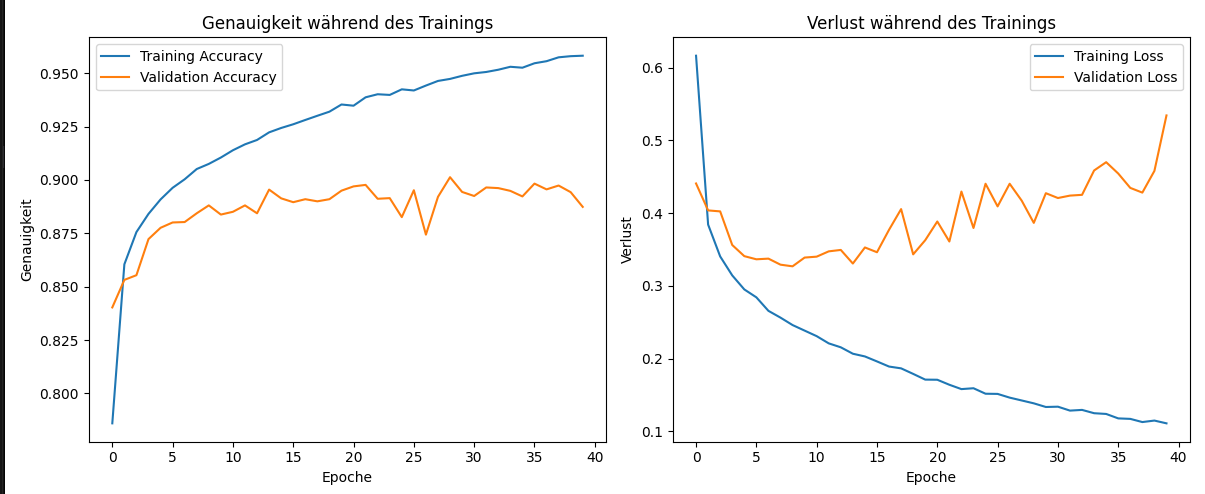
\includegraphics[width=0.8\textwidth]{image.png}
    \caption{Trainingsgenauigkeit und Verlust über die Epochen}
    \label{fig:training-curves}
\end{figure}

\section*{Evaluation}
Nach dem Training wurde das Modell auf dem Testdatensatz evaluiert. Die Ergebnisse waren:
\begin{itemize}
    \item Testverlust: 0.5342
    \item Testgenauigkeit: 88,74\%
\end{itemize}

\section*{Fazit}
Dieses Projekt hat erfolgreich ein neuronales Netzwerk zur MNIST-Ziffernklassifikation implementiert. Mit einer Testgenauigkeit von 88,74\% zeigt das Modell eine solide Leistung.

\section*{Source Code}
Der vollständige Quellcode für dieses Projekt ist auf GitHub unter folgendem Link verfügbar: \url{https://github.com/Luna-Schaetzle/INFI_Informations_Systeme/tree/main/Aufgabe_5}

\section*{References}
\begin{enumerate}
    \item MNIST Dataset: \url{http://yann.lecun.com/exdb/mnist/}
    \item MNIST Fashion Dataset: \url{https://github.com/zalandoresearch/fashion-mnist?tab=readme-ov-file}
    \item Keras Documentation: \url{https://keras.io/}
    \item TensorFlow Documentation: \url{https://www.tensorflow.org/}
    \item GitHub Repository: \url{https://github.com/Luna-Schaetzle/INFI_Informations_Systeme/tree/main/Aufgabe_5}
    \item Python Documentation: \url{https://docs.python.org/3/}
\end{enumerate}

\section*{Contact Information}
For any questions or clarifications, please contact me at \\ 
\textbf{Luna P. I. Schätzle \\}
\textbf{Email:} luna.schaetzle@gmail.com \\
\textbf{Website:} \url{https://luna-schaetzle.xyz} \\
\textbf{GitHub:} \url{https://github.com/Luna-Schaetzle}

\end{document}
